% report.tex - 

\documentclass[10pt]{report}
\usepackage[margin=2.5cm]{geometry}
\usepackage[small,labelfont=it,textfont=it]{caption}
\usepackage{graphicx, cite, url, subfig, listings, longtable, algpseudocode}

\begin{document}
\title{CS515 - Project 1: Implementation, design, and results.}
\author{Josh Reese\\00258-32334}
\maketitle

\section{Implementation}
The server submitted here implements a basic event driven
architecture. The server is structured in the following way:
\begin{algorithmic}
  \State set up socket
  \While {True}
  \State select()
  \For {$i=0 -> max\_file\_descriptors$}
  \If {$i\ set\ to\ read$}
  \If {$i == server\_socket$}
  \State accept new connection
  \State create Responder for this connection
  \Else
  \State receive on i
  \If {$receive\_is\_terminating$}
  \State close(i)
  \Else
  \State send header
  \State add Responder to the write queue
  \EndIf
  \EndIf
  \EndIf
  \If {$i\ set\ to\ write$}
  \State read Responders next chunk of data from disk
  \State send(i)
  \EndIf
  \EndFor
  \EndWhile

\end{algorithmic}
The main structure to allow this to work is a class I've
called \emph{Responder}. These class will contain all the information
the server will require to interact with a client. As clients connect
to the server Responders are created accordingly and these Responders
will allow the server to switch between connections and send smaller
chunks of data to each client. One difficult choice was whether to
read in the entire file from the disk in the beginning or to read in
chunks at a time as they were needed. It seems that for large files
this method will be much more feasible. However, with small files this
approach might introduce significant overhead. There are several files
involved the server:\\\\
{\bf myhttpd.[ch]}:\\
This is the main server code. Contains code for the algorithm
described above.\\\\
{\bf file\_handler.[ch]}:\\
As the name suggests this code handles all interactions with
files. This includes checking for any errors in the request related to
the file (e.g. file not found). In addition this will check the type
of file and get its length for use in the header. Of course the code
to read a chunk of a file is here as well. This method will also
handle making sure we don't read more of the file than what exists.\\\\
{\bf request\_handler.[ch]}:\\
The main purpose of this class is to create the header. This works by
the server calling \emph{get\_header()}. From here various checks are
made to make sure the request can be fulfilled. If the request can be
filled the server will proceed otherwise the reply will consist of the
error code, and a page letting the user know what went wrong.\\\\
{\bf Responder.[ch]}:\\
This class is a container to help the server when sending to multiple
clients at the same time. Here we track the current offset into the
file (so we know where to read from for the next send), the id of the
Responder (i.e. the socket number its using), whether or not it's
currently in the sending state, a pointer to the file\_handler
attached to the file its sending, and a time that corresponds to the
last activity from this Responder (used for HTTP/1.1).\\\\
The main design decision for 1.1 was to store records in a min-heap,
sorted on time value. The heap will contain a pair (time, Responder
id). When a Responder takes an action their time is updated. Then at
the end of each main loop for the server the heap is examined. The
first time to do is check the top value of the heap. If this value
hasn't timed out yet no one has timed out. However, if this has timed
out an arbitrary number of other elements in the heap could have timed
out as well. So, we keep popping until we come across a value that
hasn't timed out. One other thing that must happen before a Responder
has been considered timed out is, when popping values off the heap, we
need to check if this value is the same value recorded inside the
Responder. If the Responder has been active recently it will have a
newer time, so this must be updated.\\\\
The client application is very straightforward. We simply spawn a
number of threads and each makes a connection to the server. Each
thread then requests a file, receives the response and disconnects. 

\section{Results}
For the experimentation portion of this project I create a custom
topology inside of mininet. This topology simply contained 1 switch
with all the hosts connected to the switch. All tests were performed
with links with a bandwidth of 10Mb/s and a delay of 6ms. All the
tests were performed again on links of the same bandwidth but a delay
value of 24ms. The initial delay was used because this produced the
same RTT I discovered between my home server and a machine on
campus. The second value was used to simulate a congested network,
operating at 1/4 the link speed of a 'normal' network. The
organization of the tests was as follows:
\begin{itemize}
\item All tests were performed 5 times
\item There were 3 files to be requested from the server of varying
  sizes (1.3MB, 5KB, and 200B)
\item Each test used a client which would run 5 threads
\item The number of hosts were incremented from each test
  (5,25,50,100)
\end{itemize}
Several charts follow illustrated some of the times discovered in the
tests.

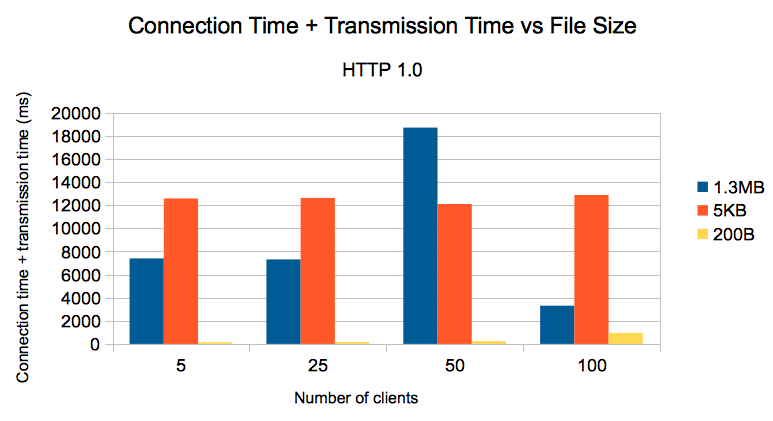
\includegraphics[scale=0.6]{images/conntran_fs_10.png}\\
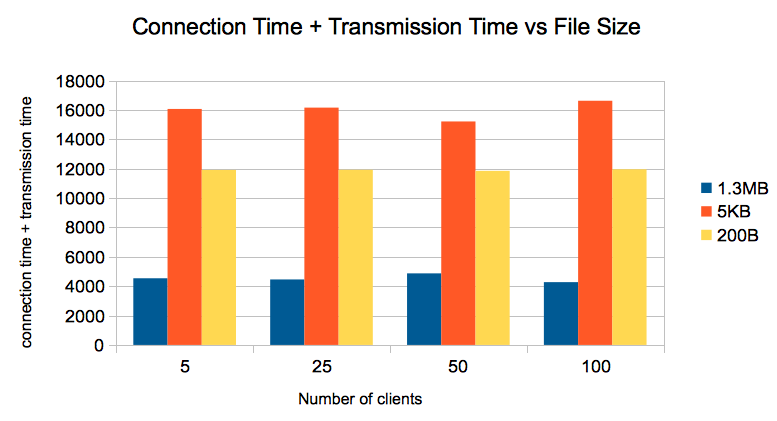
\includegraphics[scale=0.6]{images/conntran_fs_11.png}\\
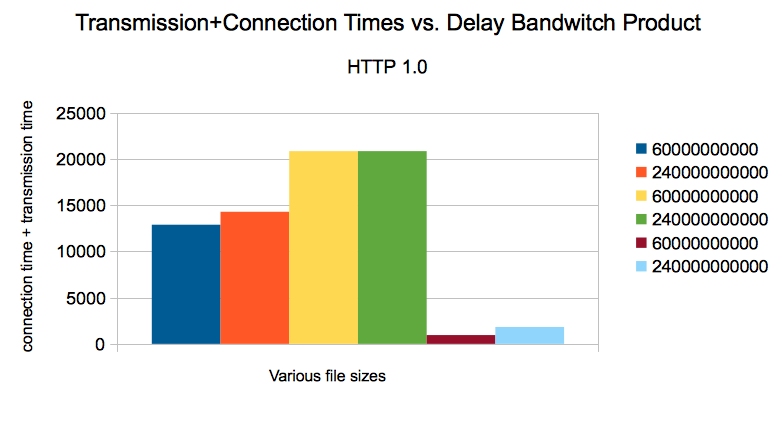
\includegraphics[scale=0.6]{images/pngconntran_del_10.png}\\
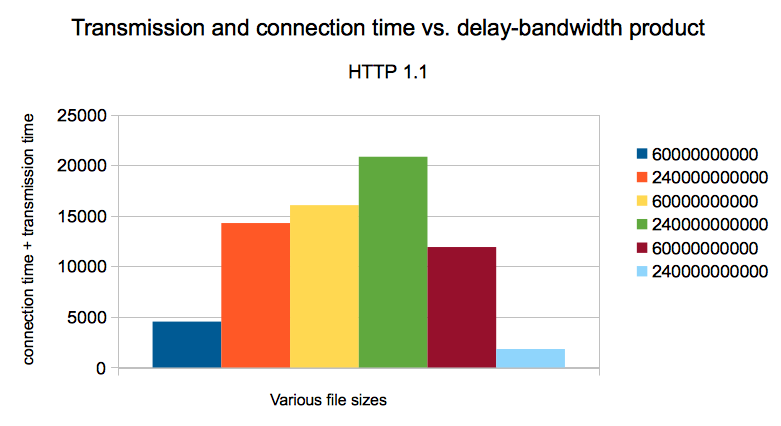
\includegraphics[scale=0.6]{images/pngconntran_del_11.png}\\
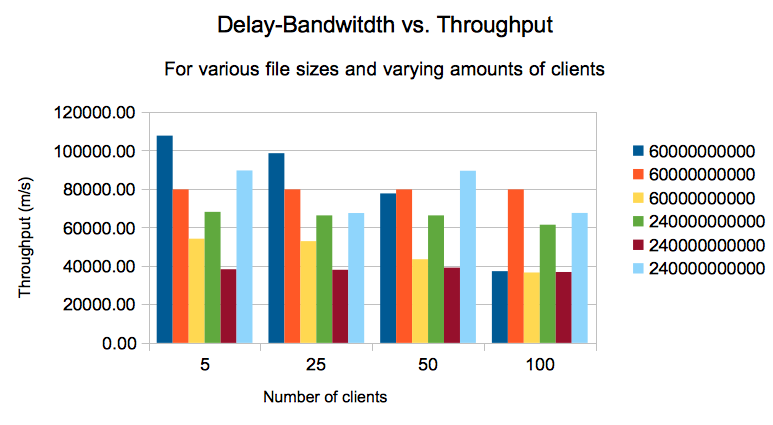
\includegraphics[scale=0.6]{images/through_delay.png}\\
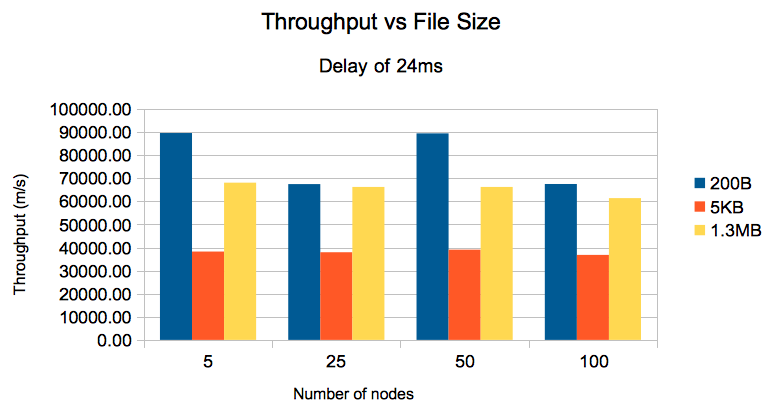
\includegraphics[scale=0.6]{images/through_size24ms.png}\\
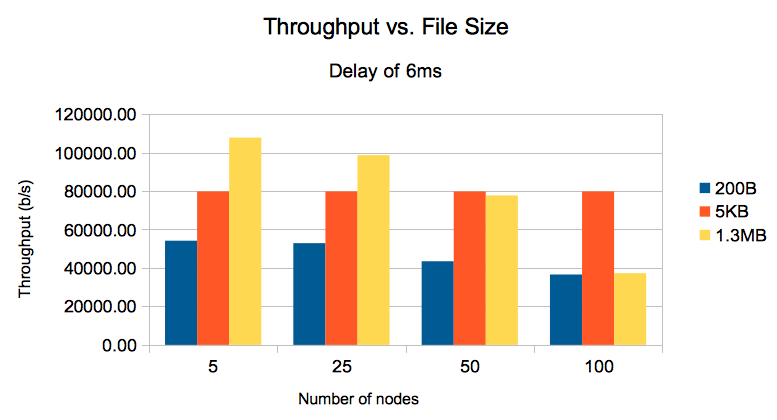
\includegraphics[scale=0.6]{images/through_size6ms.png}\\

%\bibliography{sol}{}
%\bibliographystyle{plain}
\end{document}
